

\documentclass[runningheads]{llncs}
\usepackage[utf8]{inputenc}
% \renewcommand{\baselinestretch}{1.5} 
\usepackage[english]{babel}
\usepackage[a4paper,inner=1.7cm,outer=2.7cm,top=2cm,bottom=2cm,
bindingoffset=1.2cm]{geometry}
\usepackage[
backend=biber,
style=ieee]{biblatex}
\usepackage{tabularx}
\usepackage{graphicx}
\usepackage{listings}
\usepackage[super]{nth}
\usepackage{caption}
\usepackage{multirow}
\usepackage{hhline}
\usepackage{hyperref}
\graphicspath{ {./images/} }
\usepackage{mwe}
\usepackage{float}
\usepackage[section]{placeins}
\usepackage[scaled=.92]{mathptmx}
\usepackage{microtype}
\usepackage{graphicx}
\usepackage{wrapfig}
\usepackage{enumitem}
\usepackage{enumerate}
\usepackage{fancyhdr}
\usepackage{amsmath}
\usepackage{index}
\usepackage{istgame}
\usepackage{multicol}

\usepackage{graphicx}
\addbibresource{refs.bib}




\usepackage[compact]{titlesec}         % 
\titlespacing{\section}{4pt}{4pt}{4pt} % this reduces space between (sub)sections to 0pt, for example
\AtBeginDocument{%                     % this will reduce spaces between parts (above and below) of texts within a (sub)section to 0pt, for example - like between an 'eqnarray' and text
  \setlength\abovedisplayskip{0pt}
  \setlength\belowdisplayskip{0pt}}

\begin{document}
%
\title{Negation Cue Detection using SVM and XGBoost Classifiers}
%
%\titlerunning{Abbreviated paper title}
% If the paper title is too long for the running head, you can set
% an abbreviated paper title here
%
\author{
Sergio A. Gutierrez Maury (2647606)
}
\authorrunning{Gutierrez Maury S.A}
%
% First names are abbreviated in the running head.
% If there are more than two authors, 'et al.' is used.
%
\institute{Vrije Universiteit Amsterdam}
%
\maketitle              % typeset the header of the contribution

\begin{abstract}

This paper presents a comparative study of two machine learning models, Support Vector Machines (SVM) and XGBoost, for detecting negation cues in text data. Negation cues can significantly impact the meaning of a sentence, and their accurate detection is crucial for obtaining reliable insights from text data. The study evaluates the performance of the models in detecting negation cues and their scope using an ablation analysis. The results show that both SVM and XGBoost models perform well in detecting negation cues, with SVM slightly outperforming XGBoost. The findings of this study can aid in the development of more accurate natural language processing tools for text data analysis. However, the limitations of the study, such as the imbalanced dataset, suggest the need for further research in this area.

\keywords{Support Vector Machine (SVM)  \and XGBoost \and Negation Cue Detection.}
\end{abstract}
% ----------------------------
\section{Introduction}
Negation Cue Detection is an essential aspect of Natural Language Processing (NLP) and Text Mining that enables automated systems to classify the sentiment or opinion expressed in a sentence. In essence, negation cues are linguistic markers that indicate the presence of negation in a sentence. They can manifest in diverse forms, such as single words like "never," multi-words like "no longer" and "by no means," or affixes like "im-" and "-less." Negation cues can also be complex, discontinuous, and have a scope that encompasses all negated concepts and events, excluding the negation cue itself \cite{jbara-2012}. 
\\

However, identifying negation cues presents several challenges in NLP and Text Mining. For example, negation cues can have different meanings depending on the context in which they appear, and detecting their scope can be difficult in complex sentences. Moreover, the incorrect detection or omission of negation cues can significantly impact the overall interpretation of the text, leading to unreliable insights and results.
\\

Therefore, accurately detecting negation cues is vital for many NLP and Text Mining tasks, such as Sentiment Analysis \cite{cruz2016machine} and Clinical Text Mining \cite{mehrabi2015deepen}, as it enables automated systems to extract the correct sentiment or opinion expressed in the text data. 
\\

This paper presents two models for automatic negation cue classification,  Support Vector Machines (SVM) and XGBoost, and conduct an ablation study to determine the impact of the features used in automatic detection. The study aims to assess the performance of the models in accurately detecting negation cues and their scope, which is crucial for obtaining reliable insights from text data.
\\

 The paper is structured as follows: firstly, related work in negation cue detection is reviewed. Secondly, an annotation experiment is carried out to gain a deeper knowledge in the data annotation process. Thirdly, a description of the data used in the experiments is presented. Next, the corpus pre-processing and feature extraction is described. After this, the description of the experimental setup is presented, where an ablation study is done, with its results. In section \ref{sec:error}, an error analysis is performed, with the best-performing iteration out of the ablation study, on the circle test set. Finally, the conclusions of the present research are carried out, with the main challenges and limitations discussed.


% ----------------------------
\section{Related Work \label{sec:relatedwork}}
Negation Cue detection received a lot of attention from the scientific community \cite{story2020}. For instance, Lapponi et al. (2012) \cite{lapponi2012uio} describe a system submitted by the University of Oslo to the 2012 SEM Shared Task on revolving negation. The authors based their identification of negation cues work on the light-weight classification scheme presented by Velldal et al. (2012) \cite{velldal2012speculation}, using an SVM classifier trained using simple n-gram features over words, both full forms and lemmas of the word in question and of words to the left and to the right of it.
\\

The authors added features to identify morphological or affixal cues in addition to token-level features. The first of these features records character n-grams from both the beginning and end of the base that an affix attaches to (up to five positions). The second feature targets affix cues. The authors try to emulate the effect of a lexicon look-up on the remaining substring after "subtracting" the affix, checking the status of both the remaining substring and its POS tag. 


\begin{table}[!h]
\centering
\caption{\label{tab:chowdhury} Feature set in Chowdhury et al. Negation Cue Classifier}
\begin{tabular}{ll}
\hline
Feature Name & Description \\ \hline
$POS_{i}$ & Part-of-Speech of $token_{i}$ \\
$Lemma_{i}$ & Lemma form of $token_{i}$ \\
$Lemma_{i-1}$ & Lemma form of $token_{i-1}$ \\
$hasNegPrefix$ & \begin{tabular}[c]{@{}l@{}}If $token_{i}$ has a negation prefix and is found \\ inside the automatically created vocabulary \end{tabular} \\
$hasNegSuffix$ & \begin{tabular}[c]{@{}l@{}}If $token_{i}$ has a negation suffix and is found \\ inside the automatically created vocabulary \end{tabular} \\
\textit{matchesNegExp} & If $token_{i}$ is found in \texit{NegExpList} \\

\hline
\end{tabular}
\end{table}

The authors explain the motivation behind this feature as "\textit{the occurrence of a substring such as 'un' in a token such as 'underlying' should be considered more unlikely to be a cue given that the first part of the remaining string (e.g., 'derly') would be an unlikely way to begin a word.}"

Chowdhury et al. (2012) \cite{chowdhury2012fbk} presents a system for the automatic detection of negation cues along with their scopes and corresponding negated events presented for Task 1 of the 2012 SEM Shared Task. The authors claim their approach uses comparatively fewer features than other works developed for the same task. They approach the problem as a sequence classification task, training different 1st order Conditional Random Field classifiers for each of the different sub-tasks. 
For the negation cue detection subtask, the authors automatically collect a vocabulary of all the positive tokens after excluding negation cue affixes from the training data and use them to extract features that could help to identify negation cues that are subtokens. They also create a list of highly probable negation expressions (\textit{NegExpList}) from the training data based on the frequencies. The list contains the following terms: \textit{nor, neither, without, nobody, none, nothing, never, not, no, nowhere} and  \textit{non}. Additional post-processing is done to annotate some obvious negations missed by the classifier. The final feature set for the negation cue classifier is shown in Table \ref{tab:chowdhury}

The extraction of dependency graphs and features based on this could help in modeling the syntactic relationship between each token and the closest negation cue. Jiménez-Zafra et al. (2020) \cite{jimenez2020detecting} focused their work on the detection of negation scopes and cues in Spanish, and among other features, they extracted dependency features as the dependency relation and direction between the token and the cue, and the dependency shortest path from the token in focus to the cue and vice versa. Also, Cruz et al. (2016) \cite{cruz2016machine} showed that highly accurate extraction of syntactic structure is beneficial for the negation scope detection task. Lapponi et al. (2012) \cite{lapponi2012uio} uses features defined over dependency graphs. All these works have in common the use of dependency-based features for the task of Negation Scope and Cue detection, and they have proved that the use of these types of features improves the performance of the classifiers in these tasks.

No mention was found of using the XGBoost algorithm for negation cue detection for English corpora, yet Domınguez-Mas et al. (2019) \cite{xgb2019} applied it and SVM-linear model for the Spanish dataset for negation cue detection, and it performed better than the SVM-linear model. Current research, therefore, aims to compare the performance of these two algorithms for negation cue detection in English.
% ----------------------------
\section{Data Annotation}
This section presents an inter-annotator agreement (IAA) section that aims to gain a better understanding of the annotation process of negation cues in texts related to the vaccination debate using the e-Host annotation tool. The purpose of this section is to compare, analyze, and quantify the annotations made by different annotators and to identify sources of disagreement among them, with the ultimate goal of improving the final classification.

To ensure consistency, the annotation process follows the guidelines provided by Morante et al. \cite{morante2011annotation}. Each member of the group independently annotates the same corpus of texts, which contains a mix of pro and anti-vaccination opinions from various sources, including official sources such as the National Health Service UK, as well as independent publications like the National Vaccine Information Center and Natural News.

The annotation guidelines provide possible negation cues for each part of speech and offer examples on how to determine the scope of the negation. They also include instructions on how to separate the negation scope from the rest of the phrase based on a simple grammatical analysis, which involves reformulating the phrase to test whether a part of it belongs to the scope or not. Specific rules on the separation of scope based on the part of speech that was negated are provided to minimize the annotator's bias. Special constructions such as questions and imperatives are also included in the guidelines, as well as examples of false negations and non-existing scope, to avoid expected mistakes.

Overall, this section aims to provide insights into the annotation process of negation cues and how it could impact the final classification. By comparing, analyzing, and quantifying the annotations made by different annotators, this section contributes to the understanding of the sources of disagreement and helps identify areas for improvement in the annotation process.
% All annotations were added to our \href{https://github.com/Sergi095/Applied-Text-Mining-VU-Course-2023-}{GitHub Repository}

\subsection*{Inter-Annotator Agreement Analysis}
As part of our investigation into the annotation process and its impact on the final classification, an inter-annotator agreement (IAA) analysis was conducted. In this section, we present the results of the IAA analysis and discuss the sources of disagreement among the annotators.

Each member of the group independently annotated a set of 12 texts following the guidelines provided by Morante et al. \cite{morante2011annotation}, which offered detailed instructions on how to identify negation cues and determine their scope. The purpose of the IAA analysis was to compare, analyze, and quantify the annotations made by different annotators and to identify sources of disagreement among them.

\begin{figure}[!h]
\begin{center}
  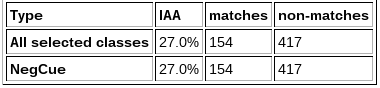
\includegraphics[width=0.6\textwidth]{Plots and results/4way.png}
  \caption{4-way IAA result}
  \label{fig:4way}
\end{center}  
\end{figure}

The results of the IAA analysis were obtained by comparing the annotations made by each member of the group. Figure \ref{fig:Pairwise agreement} shows the pair-wise agreement scores obtained from the analysis. We conducted an error analysis to systematically identify and explain the sources of disagreement among annotators. The analysis was based on a random sample of errors, and patterns were identified and illustrated with examples.

\begin{figure}[!h]
  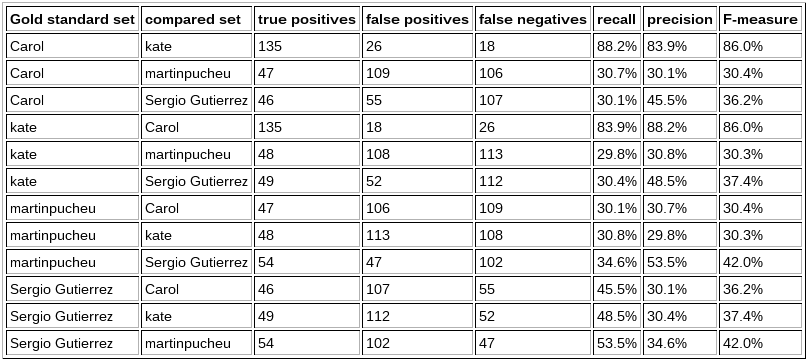
\includegraphics[width=\linewidth]{Plots and results/pairwise.png}
  \caption{Pair-wise agreement}
  \label{fig:Pairwise agreement}
\end{figure}

The results of the analysis revealed that human error and a lack of alignment between the text versions used for annotation were the main sources of disagreements among annotators. Specifically, disagreements arose when annotators failed to highlight the entire word or phrase, instead only highlighting part of it. For example, with words like "unclear", "unprotected", and "unpublished", some annotators highlighted the complete word, while others only highlighted the prefix "un". Similarly, with the word "don't", some annotators only highlighted the contraction, while others did the complete word.

To address these sources of disagreement, we suggest implementing a more thorough training process for the annotators, which could include a detailed review of the guidelines and examples, as well as further practice sessions. Moreover, we suggest that the guidelines could be further expanded to cover more examples of negation cues in different contexts to reduce ambiguity. Additionally, post-processing the annotations to annotate some obvious negations missed by the classifier would also help to improve the overall agreement scores, as shown in Figure \ref{fig:4way}.


To sum up, this section provided insights into the annotation process of negation cues. The inter-annotator agreement analysis helped to identify the sources of disagreement among the annotators and highlighted the need for more thorough training to reduce ambiguity. The results also emphasized the importance of post-processing the annotations to improve the overall agreement scores.

% ----------------------------
\section{Dataset Description}
 
Before the emergence of SEM 2012, the only dataset used for the Negation Cue Classification available was the Bioscope dataset, which was collected from medical papers, and the main objective was to build classifiers that would allow reliable interpretation of medical research. Unfortunately, the classifiers built on that dataset would generalise poorly to other texts, therefore SEM CD-SCO dataset was created in order to create a possibility to train negation cue classifiers applicable to non-scientific language. CD-SCO was built on Conan Doyle stories. Originally, CD-SCO is annotated with negation cues, scope of negation, and the event or property being negated. For this task, however, the scope and negated event or property annotations are going to be disregarded.


\begin{table}[!h]
\centering
\caption{\label{tab:tags} Annotation tag counts}
\begin{tabular}{llll}
\hline
\multicolumn{1}{c}{\textbf{Dataset}} & \multicolumn{1}{c}{\textbf{O}} & \multicolumn{1}{c}{\textbf{B-NEG}} & \multicolumn{1}{c}{\textbf{I-NEG}}                                                                                            \\ 
\hline
Training Set & 64448 & 987 & 16\\
Test Set 1 & 10049 & 134 & 1\\
Test Set 2 & 8893 & 135 & 4\\
Development Set & 13388 & 176 & 3 \\
\hline
\end{tabular}
\end{table}



Without the scope and negated property or event annotations, the dataset consists of five columns. A snippet of the dataset can be seen in Table \ref{tab:trainingdf}, representing the sentence: \textit{"Remarkable, but by no means impossible," said Holmes, smiling."}. The first column contains information about which story the token is from and which chapter. The second column represents the number of the sentence the token is taken from. The third column represents the position of the token itself in the sentence. The fourth column is the token itself. The last column represents if the token is a negation cue. If the token is not a negating one, it is marked with 'O', if it is a single-word negation cue it is marked with 'B-NEG'. If the negation consists of more than one world, for example, 'by no means', token 'no' is marked as 'B-NEG', as a main negation word, and tokens 'by' and 'means' are marked as 'I-NEG', representing their negating role in this context, while being 'O' in another context. Table \ref{tab:tags}  presents counts of each tag for Training and Development datasets.




\begin{table}[!h]
\centering
\caption{\label{tab:trainingdf}Training dataset snippet}
\begin{tabular}{ccccc}
\hline
file       & nSentence & nToken & Token        & Golden Label  \\ 
\hline
wisteria01 & 248       & ~ ~0   & ~ ~\`{}\`{}~ & O             \\
wisteria01 & 248       & 1      & Remarkable   & O             \\
wisteria01 & 248       & 2      & ,            & O             \\
wisteria01 & 248       & 3      & but          & O             \\
wisteria01 & 248       & 4      & by           & B-NEG         \\
wisteria01 & 248       & 5      & no           & I-NEG         \\
wisteria01 & 248       & 6      & means        & I-NEG         \\
wisteria01 & 248       & 7      & impossible   & B-NEG         \\
wisteria01 & 248       & 8      & ,            & O             \\
wisteria01 & 248       & 9      & ''           & O             \\
wisteria01 & 248       & 10     & said         & O             \\
wisteria01 & 248       & 11     & Holmes       & O             \\
wisteria01 & 248       & 12     & ,            & O             \\
wisteria01 & 248       & 13     & smiling      & O             \\
wisteria01 & 248       & 14     & .            & O             \\
\hline
\end{tabular}
\end{table}


% ----------------------------
\section{Corpus Pre-processing \& Feature Extraction \label{sec:featEx}}
For the Corpus Pre-Processing, given that the original corpus has been already pre-processed and tokenized, it was not possible to extract additional linguistic information from it, at least not in its tabular form. Because of this reason,the dataset was reverse-engineered, reconstructing the original sentences and applying NLP tasks over them in order to extract additional information e.g. a token's POS tag. 

Once the original sentences were reconstructed, we use the spaCy library to perform the new NLP analysis, extracting a new set of tokens for each sentence. In most cases, the spaCY tokenization and the original tokenization matched, but in some cases, these two tokenizations differed, for example with some compound words like \textit{old-fashioned} which in the original dataset is tokenized as a single token and spacy tokenize it as \textit{old}, '\textit{-}' and \textit{fashioned}. In such cases, original tokenization was preserved. 


Feature extraction plays a crucial role in building effective classifiers, as by properly extracting relevant features, NLP classifiers can achieve better accuracy and generalizability. It consists of the process of identifying and extracting relevant information from text data, which is then used as input to a machine learning algorithm.

Taking inspiration from previous research described in the related work section \ref{sec:relatedwork}, a set of features from the NLP analysis were selected, like the POS-tag and l from each token, and also the lemma from the previous token. Also, using the spaCy dependency parser and inspired by Jiménez-Zafra et al. (2020) \cite{jimenez2020detecting} a set of dependency features as the head from each sentence and the dependency label from each token to its sentence-head were extracted. The length of the path connecting each token to its head was also extracted. 

\begin{table}
\centering
\caption{\label{tab:features} Set of Features for the classifier}
\begin{tabular}{ll}
\hline
\multicolumn{1}{c}{\textbf{Feature Name}} & \multicolumn{1}{c}{\textbf{Description}}                                                                                              \\ 
\hline
POS_i                                                 & Part-of-Speech tag of token_i\\
Lemma_i                                               & Lemma form of token_i\\
Lemma_{i-1}                                           & Lemma form of token_{i-1}\\
Dependency                                            & Dependency Label from $token_{i}$ with\\& respect to its sentence root \\
Head                                                  & Sentence root\\
RootPath                                              & Length of the path from token to its root\\
hasNegAffix                                           & Token contain one of the affix from list \\
NegExpList                                            & If token is in \textit{NegExpList} \\

Token_{i} & The specific token. \\
\hline
\end{tabular}
\end{table}


The \textit{NegExpList} described by Chowdhury et al. (2012) \cite{chowdhury2012fbk} and checked each token for its presence in the list was also extracted as a feature. The list contains the following terms: \textit{nor, neither, without, nobody, none, nothing, never, not, no, nowhere} and  \textit{non}, which are only terms with a negative polarity. Additionally, a check was performed for each token containing the affixes described by Lapponi et al. (2012) \cite{lapponi2012uio}: \textit{un}, \textit{dis}, \textit{ir}, \textit{im}, and \textit{in}, and the infix and suffix \textbf{"less"}. A complete description of the extracted features is shown in Table \ref{tab:features}.

% ----------------------------
\section{Experiments}
The experimental setup consisted in an ablation approach to investigate the impact of individual features on the performance of two machine learning algorithms, namely Support Vector Machines (SVM) and XGBoost. To conduct the study, each feature in the feature set (as presented in Table \ref{tab:features}) was removed one at a time, and the models were retrained without the removed feature, as shown in table \ref{tab:ablation}. Subsequently, the performance of the models was evaluated on a validation set, which consisted of 30\% of the training set, with a stratification of the target variable. As the distribution of the target variable was imbalanced, as illustrated in Table \ref{tab:tags}, two sampling techniques were incorporated into the training pipeline.

Specifically, the pipeline involved a column preprocessor that implemented standard scaling for numeric features and TF-IDF (term frequency-inverse document frequency) vectorizer, both implementations came from he sklearn library \cite{scikit-learn}. Additionally, two sampling techniques, random oversampling for minority classes and random undersampling for majority classes, were included. The parameters for the grid search consisted of three hyperparameters per algorithm, including "max depth", which sets the maximum depth of the decision trees, which, "col sample by tree", which regulates the fraction of features to select for each tree, and "learning rate", which  influences the contribution of each classifier, for XGBoost. The hyperparameters for SVM were and "C", which  C controls the trade-off between maximizing the margin and minimizing the classification error, "kernel type", which specifies the kernel function used for transforming the input data into a higher-dimensional space, and "$\gamma$", which determines the shape of the decision boundary. 



\begin{table}[!ht]
\centering
\caption{\label{tab:ablation} Sets of Features During Ablation}
\begin{tabular}{cl}
\hline
\textbf{Iteration} & \multicolumn{1}{c}{\textbf{Set of Features}} \\
\hline
1 & hasNegAffix, Token, Dependency, Head, NegExpList, $Lemma_{i-1}$, POS, Lemma, RootPath \\
2 & hasNegAffix, Token, Dependency, Head, NegExpList, $Lemma_{i-1}$, Lemma, RootPath \\
3 & hasNegAffix, Dependency, Head, NegExpList, $Lemma_{i-1}$, Lemma, RootPath \\
4 & hasNegAffix, Head, NegExpList, $Lemma_{i-1}$, Lemma, RootPath \\
5 & hasNegAffix, NegExpList, $Lemma_{i-1}$, Lemma, RootPath \\
6 & $Lemma_{i-1}$, Lemma, hasNegAffix, RootPath \\
7 & $Lemma_{i-1}$, hasNegAffix, RootPath \\
8 & $Lemma_{i-1}$, RootPath \\
9 & $Lemma_{i-1}$ \\
\hline
\end{tabular}
\end{table}


\subsection{Support Vector Machine} 
\textbf{SVM} was first introduced by Vapnik and Cortes (1995) \cite{vapnik1995}, and was quickly recognized as one of the most successful classification algorithms. The basic idea behind the model is finding such a hyperplane between the plotted classes in a way, where the margin, i.e. the distance, between the two classes is maximized. SVM algorithms show great robustness against noise and control over-fitting \cite{robust2009}. Moreover, previous work regarding the application of SVM for negation Cue Detection, as described in the Related Work section, suggests the state-of-the-art performance of the algorithm for this task. The specific implementation of SVM used in this paper was  "\textit{thundersvm}", which make use of GPU in its computations. The library was created by Wen Zeyi et al. (2018) \cite{thundersvm}

\begin{figure}[!ht]
\centering
    \makebox[\textwidth][c]{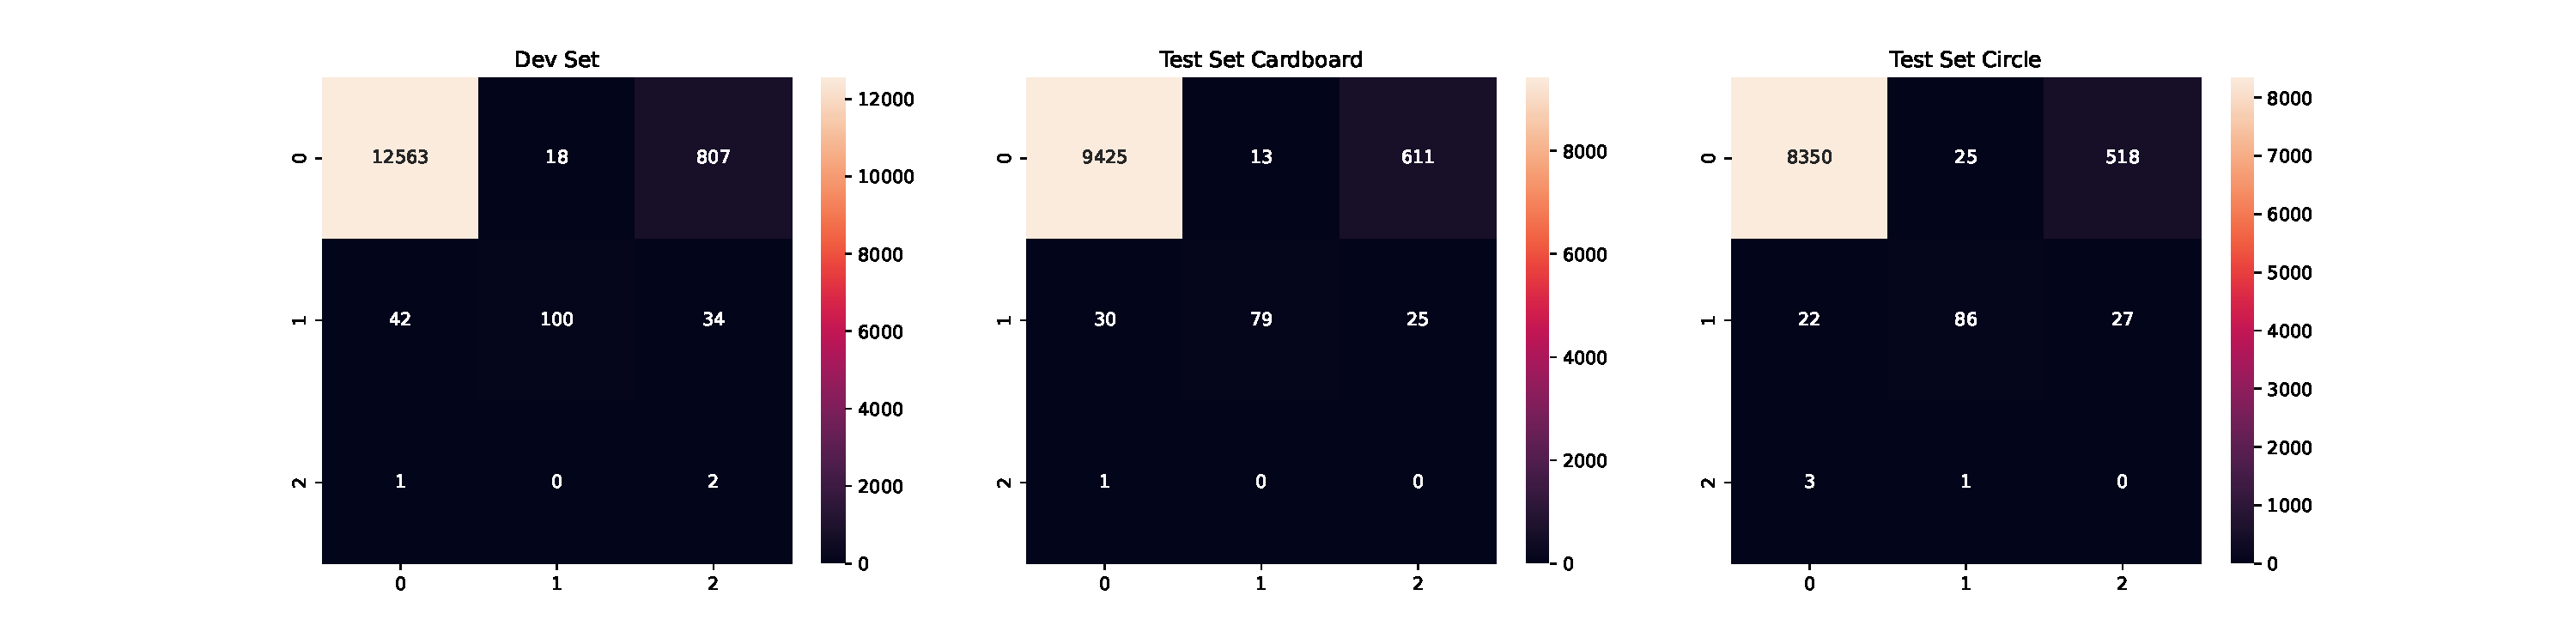
\includegraphics[width=1.3\textwidth]{Plots and results/Confusion_Matrix_base_svm.pdf}}
  \caption{Confusion Matrices Baseline SVM}
  \label{fig:base_line_svm}
\end{figure}

\subsection{XGBoost}
\textbf{XGBoost} is a powerful and complex machine learning algorithm that has shown excellent performance in capturing intricate patterns in data. As a tree-based classifier, it sequentially builds new trees upon the starting predictor tree, with each new tree aiming to predict the margin of error of the decision produced by the ensemble of trees it is built upon \cite{minasny2009elements}.

In the present research, XGBoost's tree-based classifier was implemented with the XGBoost package. The $tree\_method$ parameter was set to $gpu\_hist$ in order to decrease the running time of the algorithm. Specifically, this approach performs sketching only once and makes use of GPU, thereby enhancing computational efficiency.

\subsection{Baseline}


In an experiment designed to establish a baseline, the predictive efficacy of the token feature is assessed in isolation. In table \ref{tab:baselines_results}, the results of the baseline are depicted. It can be seen that both weighted F1-score and macro F1-score are around 0.9 and 0.5 respectively for all test sets. Figures \ref{fig:base_line_svm} and \ref{fig:base_line_xgb} shows the confusion matrices of both SVM and XGBoost on the tests and dev sets, providing a further insight into the performance with the feature token alone, it can be seen that despite not having features with contextual information, both classifiers were able to perform reasonably well.
\begin{table}[!ht]
    \centering
    \caption{Classification Report Baseline}
    \label{tab:baselines_results}
\begin{tabular}{lccc|cccr}
\hline
Dataset & \begin{tabular}[c]{@{}l@{}}Precision\\ (SVM)\end{tabular} &    \begin{tabular}[c]{@{}l@{}}Recall\\ (SVM)\end{tabular} &  \begin{tabular}[c]{@{}l@{}}F1-Score\\ (SVM)\end{tabular} & \begin{tabular}[c]{@{}l@{}}Precision\\ (XGBoost)\end{tabular} &    \begin{tabular}[c]{@{}l@{}}Recall\\ (XGBoost)\end{tabular} &  \begin{tabular}[c]{@{}l@{}}F1-Score\\ (XGBoost)\end{tabular} & Support  \\
\hline
\textbf{Cardboard} &        &        &        &       &       &       &    \\
O                  &  0.996 &  0.937 &  0.966 & 0.995 & 0.938 & 0.966 & 10049 \\
B-NEG              &  0.858 &  0.589 &  0.699 & 0.894 & 0.507 & 0.647 & 134 \\
I-NEG              &    0.0 &    0.0 &    0.0 &  0.0  & 0.0   & 0.0   & 1 \\
macro avg          &  0.618 &  0.509 &  0.555 & 0.630 & 0.481 & 0.537 & 10184 \\
weighted avg       &  0.994 &  0.933 &  0.962 & 0.994 & 0.932 & 0.961 & 10184 \\
\hline
\textbf{Circle}    &        &        &        &       &       &       &   \\
O                  &  0.997 &  0.938 &  0.967 & 0.995 & 0.940 & 0.967 & 8893 \\
B-NEG              &  0.767 &  0.637 &  0.696 & 0.850 & 0.548 & 0.667 & 135 \\
I-NEG              &    0.0 &    0.0 &    0.0 &  0.0  & 0.0   &   0.0 & 4 \\
macro avg          &  0.588 &  0.525 &  0.554 & 0.615 & 0.496 & 0.544 & 9032 \\
weighted avg       &  0.993 &  0.934 &  0.962 & 0.992 & 0.934 & 0.962 & 9032 \\
\hline
\textbf{Dev set}   &        &        &        &       &       & &   \\
O                  &  0.996 &  0.938 &  0.966 & 0.995 & 0.939 & 0.966 & 13388 \\
B-NEG              &  0.847 &  0.568 &  0.966 & 0.925 & 0.494 & 0.966 & 176 \\
I-NEG              &  0.002 &  0.667 &  0.004 & 0.002 & 0.667 & 0.004 & 3 \\
macro avg          &  0.615 &  0.724 &  0.550 & 0.641 & 0.700 & 0.538 & 13567 \\
weighted avg       &  0.994 &  0.933 &  0.962 & 0.994 & 0.933 & 0.962 & 13567 \\
\hline
\end{tabular}
\end{table}
Furthermore, the hyperparameters selected for XGBoost were $colsample \ bytree = 0.6$, $learning \ rate = 0.3$, and $max \ depth = 3$ while for SVM, the parameters were $C = 10.0$, $\gamma = 0.5$, and kernel type was set to polynomial based on the grid search results in this particular experiment.

\begin{figure}[!h]
\centering
    \makebox[\textwidth][c]{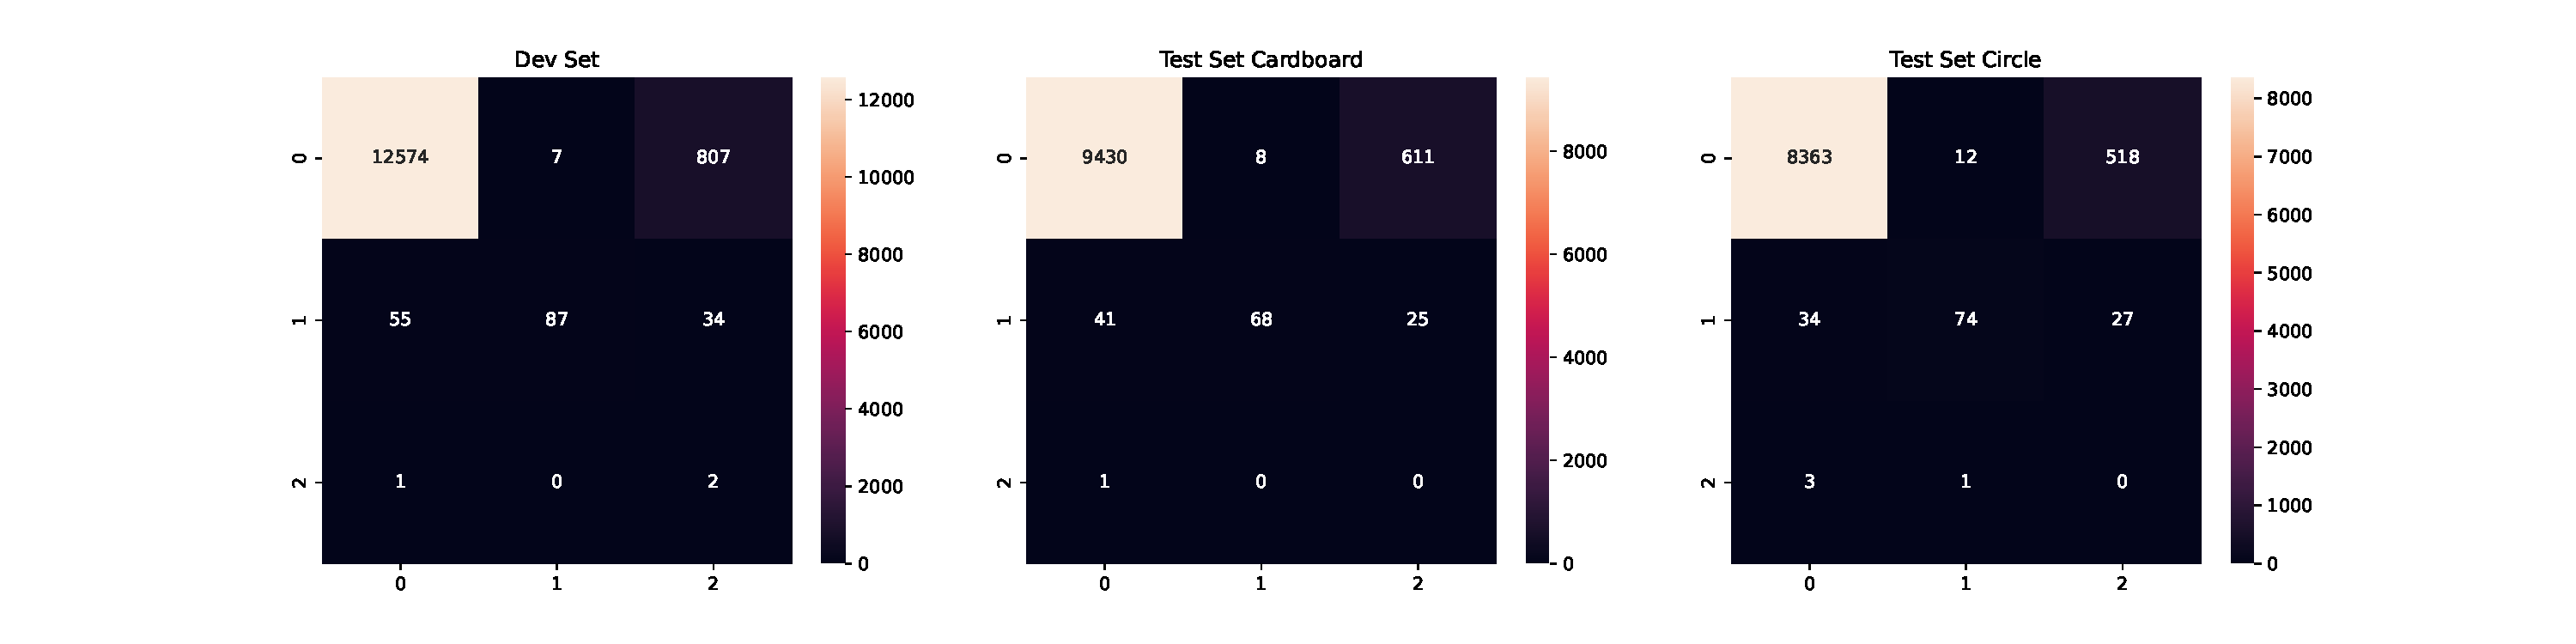
\includegraphics[width=1.3\textwidth]{Plots and results/Confusion_Matrix_base_xgb.pdf}}
  \caption{Confusion Matrices Baseline XGBoost}
  \label{fig:base_line_xgb}
\end{figure}
\subsection{Classification Experiments}

During the ablation study, a random feature was removed at each iteration, and the performance of the classifiers was evaluated. The best-performing iterations, denoted as iteration 1 for SVM (SVM 1) and iteration 2 for XGBoost (XGBoost 2), were selected based on their weighted F1-score, which provides a harmonic-weighted average of precision and recall. The weighted F1-score is an appropriate choice as it considers both the balance between precision and recall and the contribution of each class, making it suitable for evaluating classification performance in the presence of imbalanced datasets.

\begin{figure}[!ht]
\centering
    \makebox[\textwidth][c]{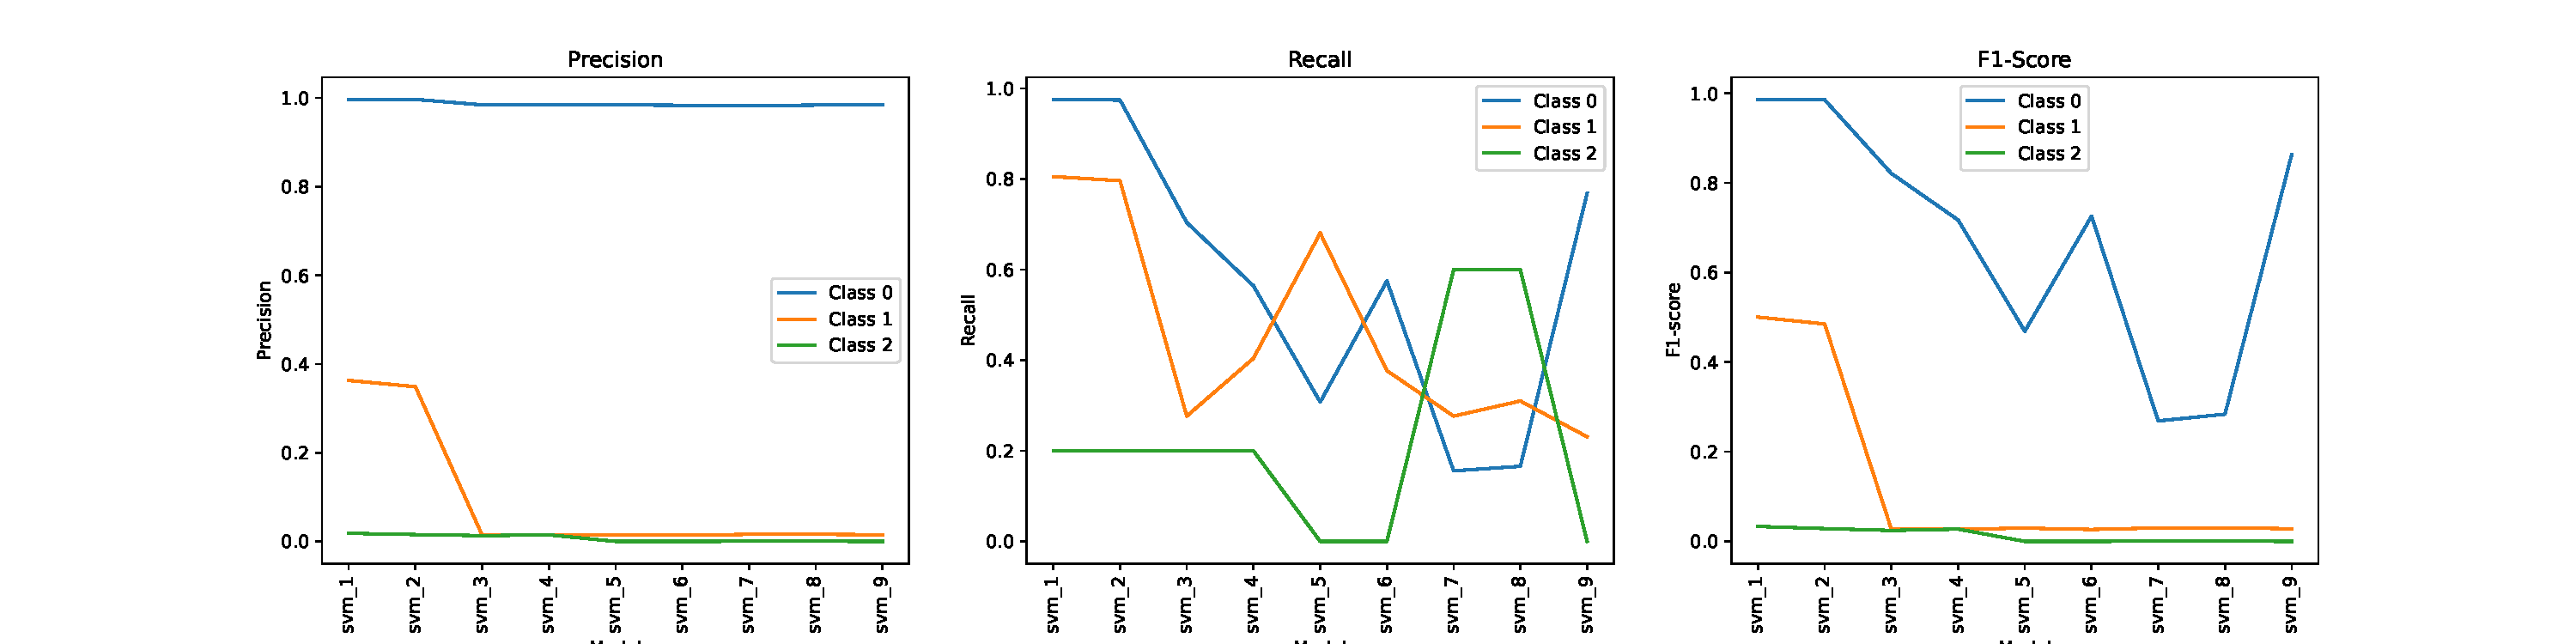
\includegraphics[width=1.3\textwidth]{Plots and results/metrics_svm_training.pdf}}
  \caption{Metrics During Ablation Study SVM}
  \label{fig:metrics_svm_training}
\end{figure}

Table \ref{tab:results} presents the classification reports for the best-performing Support Vector Machine (SVM) and XGBoost iterations. Notably, the removal of the feature Token had a remarkable impact on the performance of the classifiers, as evident from the observed drop in F1-scores in Figures \ref{fig:metrics_svm_training} and \ref{fig:metrics_xgb_training}, this drop in performance is completely understandable since the feature "token" is the negation cue itself. By examining the weighted F1-scores and confusion matrices in figures \ref{fig:best_svm} and \ref{fig:best_xgb}, it can be inferred that the SVM classifier slightly outperformed the XGBoost classifier, correctly classifying more data points. However, the SVM classifier failed to classify the minority class "I-NEG" accurately in the development set.

\begin{table}[!ht]
    \centering
    \caption{Classification Report Best Performing Model}
    \label{tab:results}
\begin{tabular}{lccc|cccr}
\hline
Dataset & \begin{tabular}[c]{@{}l@{}}Precision\\ (SVM 1)\end{tabular} &    \begin{tabular}[c]{@{}l@{}}Recall\\ (SVM 1)\end{tabular} &  \begin{tabular}[c]{@{}l@{}}F1-Score\\ (SVM 1)\end{tabular} & \begin{tabular}[c]{@{}l@{}}Precision\\ (XGBoost 2)\end{tabular} &    \begin{tabular}[c]{@{}l@{}}Recall\\ (XGBoost 2)\end{tabular} &  \begin{tabular}[c]{@{}l@{}}F1-Score\\ (XGBoost 2)\end{tabular} & Support  \\
\hline
\textbf{Cardboard} &        &        &        &       &       &       &    \\
O                  & 0.996  &  0.978 & 0.987  & 0.995 & 0.967 & 0.981 & 10049 \\
B-NEG              &  0.342 &  0.731 &  0.466 & 0.244 & 0.686 & 0.360 & 134 \\
I-NEG              &    0.0 &    0.0 &    0.0 &  0.0  & 0.0   & 0.0   & 1 \\
macro avg          &  0.446 &  0.570 &  0.484 & 0.413 & 0.551 & 0.447 & 10184 \\
weighted avg       &  0.987 &  0.975 &  0.980 & 0.985 & 0.963 & 0.973 & 10184 \\
\hline
\textbf{Circle}    &        &        &        &       &       &       &   \\
O                  &  0.996 &  0.974 &  0.985 & 0.995 & 0.959 & 0.977 & 8893 \\
B-NEG              &  0.336 &  0.785 &  0.471 & 0.220 & 0.718 & 0.337 & 135 \\
I-NEG              &    0.0 &    0.0 &    0.0 &  0.0   & 0.0   &   0.0 & 4 \\
macro avg          &  0.444 &  0.586 &  0.485 & 0.405 & 0.559 & 0.438 & 9032 \\
weighted avg       &  0.986 &  0.971 &  0.9772 & 0.984 & 0.955 & 0.9672 & 9032 \\
\hline
\textbf{Dev set}   &        &        &        &       &       & &   \\
O                  &  0.995 &  0.980 &  0.988 & 0.995 & 0.969 & 0.982 & 13388 \\
B-NEG              &  0.340 &  0.704 &  0.988 & 0.228 & 0.664 & 0.982 & 176 \\
I-NEG              &  0.0   &  0.0   &  0.0   & 0.043 & 0.333 & 0.076 & 3 \\
macro avg          &  0.445 &  0.561 &  0.482 & 0.422 & 0.655 & 0.466 & 13567 \\
weighted avg       &  0.987 &  0.976 &  0.981 & 0.985 & 0.964 & 0.973 & 13567 \\
\hline
\end{tabular}
\small

{Note:} SVM 1 and XGBoost 2 are for SVM iteration 1 and XGBoost iteration 2 of the ablation study. Table \ref{tab:ablation} presents the features with which these algorithms were trained.
\end{table}



\begin{figure}[!ht]
\centering
    \makebox[\textwidth][c]{\includegraphics[width=1.3\textwidth]{Plots and results/metrics_xgb_training.pdf}}
  \caption{Metrics During Ablation Study XGBoost}
  \label{fig:metrics_xgb_training}
\end{figure}

The optimal hyperparameters for the SVM and XGBoost classifiers were determined using grid search. For the SVM classifier, the best parameters were found to be: $ C = 1.0 $, $ \gamma = 1 $, and $ kernel = linear $.  For the XGBoost classifier, the optimal parameters were: $col \ sample \ bytree= 1.0$, $learning \ rate = 0.1$, and $max \ depth = 5$.

Comparing these results to the baseline, the results indicate that, in terms of weighted F1-score, the token feature alone performed slightly worse, which suggests that the inclusion of additional features was a beneficial modification. A closer examination of the confusion matrices reveals an increased number of accurate predictions for the majority classes in the dataset, when adding the extra features. However, he token feature alone demonstrated higher performance at the macro F1-score level.
% ----------------------------
\section{Error Analysis \label{sec:error}}
A qualitative error analysis was conducted on the predictions made by both the XGBoost 2 and SVM 1 models to gain insight into their capabilities and weaknesses when applied to the SEM 2012 circle test set. Performing such an analysis is crucial when building a negation classifier due to the complex semantic nature of negation, which interacts with various aspects of meaning and sentence structure \cite{hossain2020predicting, cruz2016machine}.
\begin{figure}[!h]
\centering
    \makebox[\textwidth][c]{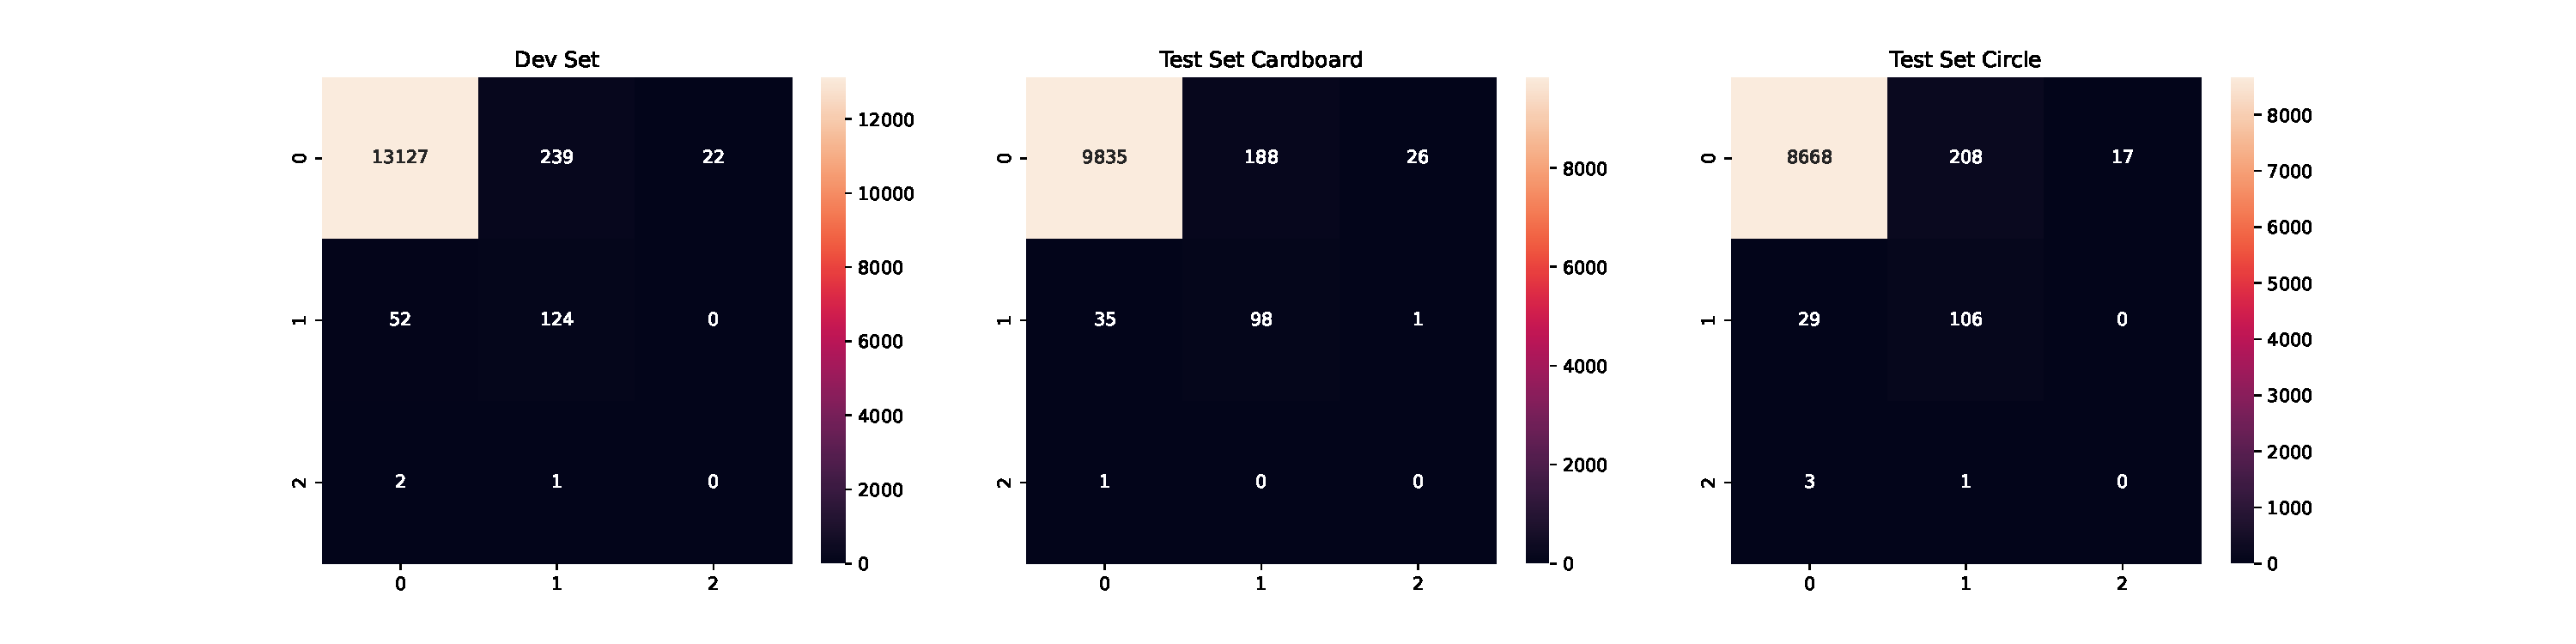
\includegraphics[width=1.3\textwidth]{Plots and results/Confusion_Matrix_svm.pdf}}
  \caption{Confusion Matrices Best Selected SVM}
  \label{fig:best_svm}
\end{figure}


\begin{table}[!h]
\caption{\label{tab:fns}Sample of false negatives in test set predictions}
\centering
\begin{tabular}{ccccc}
\hline
                                        Sentence &    Token & Golden Label & \begin{tabular}[c]{@{}l@{}}Prediction\\ (SVM)\end{tabular} & \begin{tabular}[c]{@{}l@{}}Prediction\\ (XGBoost)\end{tabular} \\
\hline
                  `` I do n't understand that . &      n't &  B-NEG &              O &              O \\
       You do n't object to tobacco , I take it ? &      n't &  B-NEG &              O &              O \\
                      I ca n't sleep for fright . &      n't &  B-NEG &              O &              O \\
                     `` I 'll have no more of it ! &     more &  I-NEG &              O &              O \\
                    That ca n't be all , Watson ? &      n't &  B-NEG &              O &              O \\
 ` If not , I 'll have no more to do with you . ' &     more &  I-NEG &              O &              O \\
         At first I thought that it was dislike . &  dislike &  B-NEG &              O &              O \\
\hline
\end{tabular}
\end{table}
Examining the false positive (FP) and false negative (FN) errors is particularly informative. An FP error occurs when the classifier identifies a negative cue token that is not annotated as such in the dataset, while an FN error takes place when the system fails to identify a token annotated as a negative cue.

\begin{table}[!h]
    \centering
    \caption{\label{tab:fps}Sample of false positives in test set predictions}
\begin{tabular}{ccccc}
\hline
                                          Sentence &      Token & Golden Label & \begin{tabular}[c]{@{}l@{}}Prediction\\ (SVM 1)\end{tabular} & \begin{tabular}[c]{@{}l@{}}Prediction\\ (XGBoost 2)\end{tabular} \\
\hline
           It sounds plausible , does it not ? &        not &      O &          B-NEG &          B-NEG \\
       Yes , here we are -- three days later . &       days &      O &          B-NEG &          B-NEG \\
      `` No doubt , sir ; but this is different . &         No &      O &          B-NEG &          B-NEG \\
      `` No doubt , sir ; but this is different . &          . &      O &          B-NEG &          B-NEG \\
         Then comes something much more definite : &  something &      O &          B-NEG &          B-NEG \\
  `` That was bad enough , but worse was to come . &       come &      O &          I-NEG &          I-NEG \\
                       One A , two B , and so on . &        and &      O &          B-NEG &          B-NEG \\
                    One A , two B , and so on . &         so &      O &          B-NEG &          B-NEG \\
                             You will hear soon . &        You &      O &          B-NEG &          B-NEG \\
                             You will hear soon . &       hear &      O &          B-NEG &          B-NEG \\
                                Is it not so ? '' &         '' &      O &          B-NEG &          B-NEG \\
              Your presence here was desirable . &          . &      O &          B-NEG &          B-NEG \\
 It was fear -- a deep , secret , shrinking fear . &     secret &      O &          B-NEG &          B-NEG \\

\hline
\end{tabular}
\end{table}
For XGBoost, the FP errors include 341 instances of B-NEG and 16 instances of I-NEG when the golden label is O. In comparison, SVM has 208 FP errors for B-NEG and 17 for I-NEG with the golden label as O. On the other hand, FN errors for XGBoost consist of 38 instances where the prediction is O, and the golden label is B-NEG, and 3 instances where the golden label is I-NEG. SVM presents a similar distribution with 29 FN errors for B-NEG and 3 for I-NEG when the model prediction is O, as seen in figures \ref{fig:best_svm} and \ref{fig:best_xgb}.

The errors observed in the test set predictions, as illustrated in tables \ref{tab:fns} and \ref{tab:fps}, could be attributed to both the complexity of negation, such as token \textit{n't}, which Cruz et al. (2016) \cite{cruz2016machine} defines as incorrect classification of a \textit{multiword cue}, and the distribution of the target variable. The current research utilized SVM and XGBoost models that incorporated semantic and syntactic features to account for this complexity, but some errors remained. Additionally, despite implementing methods to counteract the class imbalance issue in the training data, there were still insufficient examples for the algorithms to effectively learn from, which may have contributed to these persisting misclassifications.

To address these errors and improve the classifier's performance, additional data could be added to both the training set and test set to balance the distribution of the target variable. This would help reduce the problem of class imbalance in the dataset, leading to better model generalization.

\begin{figure}[!h]
\centering
    \makebox[\textwidth][c]{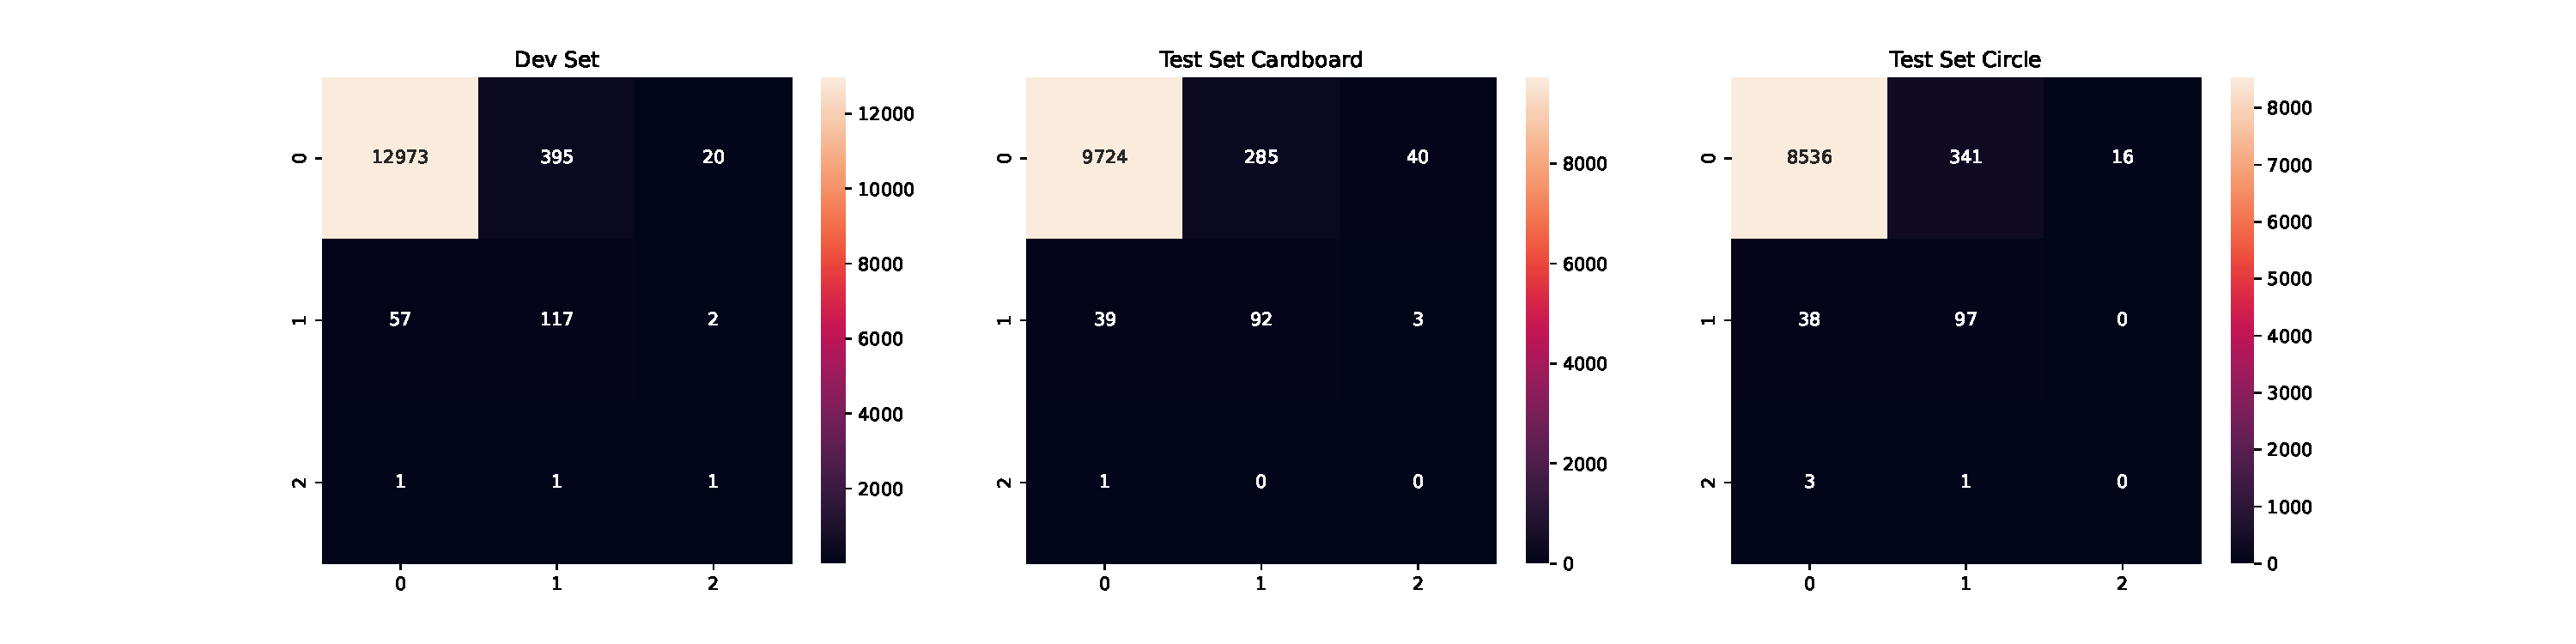
\includegraphics[width=1.3\textwidth]{Plots and results/Confusion_Matrix_xgb.pdf}}
  \caption{Confusion Matrices Best Selected XGBoost}
  \label{fig:best_xgb}
\end{figure}


% ----------------------------
\section{Conclusions}
To conclude, This paper presented the development of two machine learning algorithms, namely XGBoost and SVM, 





In conclusion, this study presented the development of a machine learning-based negation detection system, using a combination of lexical, syntactic, and semantic features. The system was evaluated on the SEM 2012 circle test set, and the results showed that both SVM and XGBoost models achieved high accuracy and F1 score, with SVM performing slightly better.


However, the error analysis revealed some limitations and weaknesses of the models in handling complex negation cases, such as multi-word cues and context-dependent negation. These findings suggest that further research is necessary to improve the models' capabilities, such as exploring more advanced features, incorporating contextual information, and utilizing more extensive training datasets.


Nonetheless, the developed system has significant potential applications in various fields, including natural language processing, sentiment analysis, and medical text analysis. For example, in medical text analysis, the ability to detect negation can help identify the absence of medical conditions or treatments, which can be critical in improving patient safety and care.


Overall, this study contributes to the development of robust and effective negation detection systems, which can benefit various applications in natural language processing and text analysis.
% ---------------------------- 
\newpage
\printbibliography


\appendix
\section{Appendix}
The code of the experiments can be found in the new repository for this project.

Link to the repository: \href{https://github.com/Sergi095/Applied_text_mining_VU_2023.git}{Negation Cue Detection using SVM and XGBoost Classifiers (ATM VU 2023)}



\end{document}



 

